\documentclass[12pt,a4paper]{article}

\usepackage[a4paper,margin=25mm]{geometry}
\usepackage{amsmath,amssymb}
\usepackage{graphicx}
\usepackage{xcolor}
\usepackage{hyperref}
\usepackage{float}
\usepackage{listings}
\usepackage{xepersian}

\settextfont{Arial}
\setlatintextfont{Consolas}
\setdigitfont{Arial}

\hypersetup{
  colorlinks=true,
  linkcolor=blue,
  urlcolor=blue
}

\definecolor{codebg}{RGB}{248,248,248}
\definecolor{codeframe}{RGB}{210,210,210}
\definecolor{codecomment}{RGB}{0,110,70}
\definecolor{codestring}{RGB}{150,40,40}
\definecolor{codekeyword}{RGB}{0,70,150}

\lstdefinestyle{pythonstyle}{
  language=Python,
  backgroundcolor=\color{codebg},
  frame=single,
  rulecolor=\color{codeframe},
  basicstyle=\small\ttfamily,
  keywordstyle=\color{codekeyword}\bfseries,
  commentstyle=\color{codecomment},
  stringstyle=\color{codestring},
  numbers=left,
  numberstyle=\tiny\color{gray},
  stepnumber=1,
  numbersep=8pt,
  showstringspaces=false,
  breaklines=true,
  tabsize=4,
  captionpos=b
}

\title{مستند الگوریتم تخمین مکان Access Point از داده‌های RSS}
\author{استخراج‌شده از کدهای موجود در پروژه}
\date{\today}

\begin{document}
\maketitle
\tableofcontents
\newpage

\section{خلاصه}
در این پروژه مکان یک اکسس‌پوینت وای‌فای از روی نمونه‌های RSS تخمین زده می‌شود.
زنجیره‌ی کد فعلی از جدول محوری زیر استفاده می‌کند:
\begin{latin}
\begin{verbatim}
data/pivot_signal_table.csv
\end{verbatim}
\end{latin}
اسکریپت اصلی تخمین مکان، فایل
\lr{03\_fit\_selected\_ap\_location.py}
است. دو فایل قبلی برای انتخاب AP و رسم نمونه‌های خام به کار می‌روند.
فایل
\lr{faculty\_map\_json.py}
برای خواندن نقشه و تبدیل مختصات جغرافیایی به مختصات محلی متری استفاده شده است.

\section{فایل‌های درگیر در الگوریتم}
\begin{itemize}
  \item \lr{01\_select\_access\_point.py}: انتخاب AP هدف با BSSID ثابت، حذف نمونه‌های نامعتبر و ذخیره‌ی آمار اولیه.
  \item \lr{02\_plot\_selected\_ap\_from\_pivot.py}: خواندن AP انتخاب‌شده و رسم نقشه‌ی شدت RSS.
  \item \lr{03\_fit\_selected\_ap\_location.py}: برازش مدل افت مسیر و تخمین مکان AP.
  \item \lr{faculty\_map\_json.py}: خواندن فایل نقشه و رسم مرز فضاهای طبقه.
\end{itemize}

\section{داده ورودی و AP هدف}
در کد، AP هدف با شناسه‌ی زیر انتخاب شده است:
\begin{latin}
\begin{verbatim}
BSSID = b28ba99a8d2a
RSS column = signal_b28ba99a8d2a
\end{verbatim}
\end{latin}
هر سطر جدول شامل مختصات نمونه‌برداری
\lr{lat, lon}
و مقدار RSS برای APهای مختلف است. مقدار
\lr{-100 dBm}
در این پروژه به‌عنوان مقدار نامعتبر یا دیده‌نشدن AP در نظر گرفته شده و نمونه‌های معتبر با شرط زیر انتخاب می‌شوند:
\[
r_i > -100.
\]
برای AP هدف، تعداد نمونه‌های معتبر برابر
\lr{1069}
است. آمار RSS استخراج‌شده از خروجی فعلی پروژه چنین است:
\[
\min r_i=-98,\qquad
\bar r=-72.8943,\qquad
\max r_i=-29.
\]

\section{مختصات محلی متری}
چون بهینه‌سازی مکانی باید برحسب متر انجام شود، مختصات جغرافیایی نمونه‌ها به مختصات محلی تبدیل می‌شود. اگر
\((\phi_i,\lambda_i)\)
به‌ترتیب عرض و طول جغرافیایی نمونه‌ی
\(i\)
باشد و
\((\phi_0,\lambda_0)\)
مبدأ محلی باشد، کد از تقریب زیر استفاده می‌کند:
\[
x_i=(\lambda_i-\lambda_0)\,111320\cos(\phi_0),
\]
\[
y_i=(\phi_i-\phi_0)\,111320.
\]
در این روابط زاویه‌ی
\(\phi_0\)
در تابع کسینوس برحسب رادیان محاسبه می‌شود و
\(x_i,y_i\)
برحسب متر هستند. در مرحله‌ی برازش، مبدأ محلی میانگین مختصات نمونه‌های معتبر است:
\[
\phi_0=\frac{1}{N}\sum_{i=1}^{N}\phi_i,\qquad
\lambda_0=\frac{1}{N}\sum_{i=1}^{N}\lambda_i.
\]

\section{مدل ریاضی RSS}
مدل به‌کاررفته در کد، مدل لگاریتمی افت مسیر است:
\[
\hat r_i = P_{1m} - 10\,n\,\log_{10}(d_i),
\]
که در آن:
\begin{itemize}
  \item \(\hat r_i\): RSS پیش‌بینی‌شده در نقطه‌ی نمونه‌ی \(i\)،
  \item \(P_{1m}\): RSS مدل در فاصله‌ی یک متر،
  \item \(n\): توان افت مسیر یا \lr{path-loss exponent}،
  \item \(d_i\): فاصله‌ی نمونه‌ی \(i\) تا مکان مجهول AP.
\end{itemize}
اگر مکان AP در دستگاه مختصات محلی برابر
\(\mathbf{a}=(a_x,a_y)\)
باشد، فاصله به شکل زیر محاسبه می‌شود:
\[
d_i=\max\left(\sqrt{(x_i-a_x)^2+(y_i-a_y)^2},\,1\right).
\]
عبارت
\(\max(\cdot,1)\)
در کد برای جلوگیری از فاصله‌ی صفر و ناپایداری
\(\log_{10}(0)\)
است.

\section{بردار پارامترها}
پارامترهای مجهول مدل عبارت‌اند از:
\[
\boldsymbol{\theta} =
\begin{bmatrix}
a_x & a_y & P_{1m} & n
\end{bmatrix}^{T}.
\]
هدف الگوریتم پیدا کردن مکان AP یعنی
\((a_x,a_y)\)
همراه با دو پارامتر رادیویی
\(P_{1m}\)
و
\(n\)
است.

\section{تابع باقیمانده و تابع هزینه}
برای هر نمونه، باقیمانده‌ی مدل به صورت اختلاف RSS پیش‌بینی‌شده و RSS مشاهده‌شده تعریف می‌شود:
\[
e_i(\boldsymbol{\theta})=\hat r_i(\boldsymbol{\theta})-r_i.
\]
در کد، این بردار باقیمانده به تابع
\lr{scipy.optimize.least\_squares}
داده می‌شود:
\[
\mathbf{e}(\boldsymbol{\theta}) =
\begin{bmatrix}
e_1 & e_2 & \cdots & e_N
\end{bmatrix}^{T}.
\]
گزینه‌ی
\lr{loss="soft\_l1"}
استفاده شده است. در پیاده‌سازی SciPy، این loss به صورت robust عمل می‌کند و اثر نمونه‌های پرت را نسبت به کمترین مربعات معمولی کاهش می‌دهد. با مقدار پیش‌فرض
\lr{f\_scale=1}
تابع هزینه‌ی مؤثر را می‌توان به شکل زیر نوشت:
\[
\min_{\boldsymbol{\theta}}
\frac{1}{2}\sum_{i=1}^{N}
2\left(\sqrt{1+e_i(\boldsymbol{\theta})^2}-1\right).
\]

\section{مقداردهی اولیه}
کد از مختصات ground-truth برای شروع بهینه‌سازی استفاده نمی‌کند. مقدار اولیه‌ی مکان AP از نقطه‌ای گرفته می‌شود که بیشترین RSS را برای AP هدف داشته است:
\[
i^\star=\arg\max_i r_i,
\]
\[
a_x^{(0)}=x_{i^\star},\qquad
a_y^{(0)}=y_{i^\star}.
\]
دو پارامتر دیگر چنین مقداردهی می‌شوند:
\[
P_{1m}^{(0)}=\operatorname{percentile}_{95}(r_i),
\qquad
n^{(0)}=2.
\]
در خروجی فعلی پروژه، مختصات نمونه‌ی شروع برابر است با:
\[
\phi_{\text{init}}=36.3127978,\qquad
\lambda_{\text{init}}=59.5263734.
\]

\section{قیود بهینه‌سازی}
برای جلوگیری از جواب‌های غیرواقعی، کد روی پارامترها کران می‌گذارد:
\[
x_{\min}-30 \le a_x \le x_{\max}+30,
\]
\[
y_{\min}-30 \le a_y \le y_{\max}+30,
\]
\[
-95 \le P_{1m} \le -20,
\]
\[
0.5 \le n \le 6.
\]
این قیود مکان AP را در محدوده‌ای نزدیک به نقاط نمونه‌برداری نگه می‌دارند و همچنین مقدار توان افت مسیر را در بازه‌ای فیزیکی‌تر محدود می‌کنند.

\section{تبدیل جواب به عرض و طول جغرافیایی}
پس از تخمین
\((\hat a_x,\hat a_y)\)،
کد آن را دوباره به عرض و طول جغرافیایی تبدیل می‌کند:
\[
\hat\phi=\phi_0+\frac{\hat a_y}{111320},
\]
\[
\hat\lambda=\lambda_0+
\frac{\hat a_x}{111320\cos(\phi_0)}.
\]

\section{معیارهای ارزیابی}
مختصات واقعی AP در کد فقط برای ارزیابی استفاده شده است، نه برای برازش:
\[
\phi_{\text{gt}}=36.312805555555556,
\qquad
\lambda_{\text{gt}}=59.52636111111111.
\]
خطای مکانی برحسب متر با فاصله‌ی اقلیدسی در مختصات محلی محاسبه می‌شود:
\[
E_{\text{loc}}=
\sqrt{(\hat a_x-a_{x,\text{gt}})^2+(\hat a_y-a_{y,\text{gt}})^2}.
\]
همچنین خطاهای RSS چنین محاسبه شده‌اند:
\[
\operatorname{RMSE}=
\sqrt{\frac{1}{N}\sum_{i=1}^{N}(\hat r_i-r_i)^2},
\]
\[
\operatorname{MAE}=
\frac{1}{N}\sum_{i=1}^{N}|\hat r_i-r_i|.
\]

\section{نتیجه‌ی اجرای فعلی}
مطابق فایل
\lr{outputs\_rss\_ap/03\_fit\_summary.json}
نتیجه‌ی اجرای فعلی چنین است:
\begin{latin}
\begin{verbatim}
estimated_lat  = 36.31281061763301
estimated_lon  = 59.5263414104742
ground_truth   = (36.312805555555556, 59.52636111111111)
location error = 1.8548439013658915 m
rss_1m_dbm     = -28.360791718620668
path_loss_n    = 3.216816335532521
RMSE           = 8.53347351228568 dB
MAE            = 6.907841020902214 dB
optimizer      = success, ftol termination condition is satisfied
\end{verbatim}
\end{latin}

\section{شبه‌کد الگوریتم}
\begin{latin}
\begin{verbatim}
Input:
  pivot_signal_table.csv
  target BSSID = b28ba99a8d2a

1. Read pivot RSS table.
2. Select RSS column signal_b28ba99a8d2a.
3. Keep samples whose RSS is greater than -100 dBm.
4. Convert sample lat/lon values to local meter coordinates.
5. Choose the strongest RSS sample as the initial AP position.
6. Initialize:
     ap_x, ap_y = strongest sample position
     rss_1m     = 95th percentile of RSS
     n          = 2
7. Define log-distance model:
     predicted_rss = rss_1m - 10 n log10(max(distance, 1 m))
8. Minimize robust residuals with scipy least_squares and soft_l1 loss.
9. Convert estimated local AP position back to lat/lon.
10. Compare against ground-truth coordinate only for reporting error.
11. Save summary JSON and draw final map.
\end{verbatim}
\end{latin}

\section{نقشه‌ها}
اگر تصاویر خروجی در پوشه‌ی
\lr{figures}
موجود باشند، در این بخش وارد می‌شوند.
\begin{figure}[H]
  \centering
  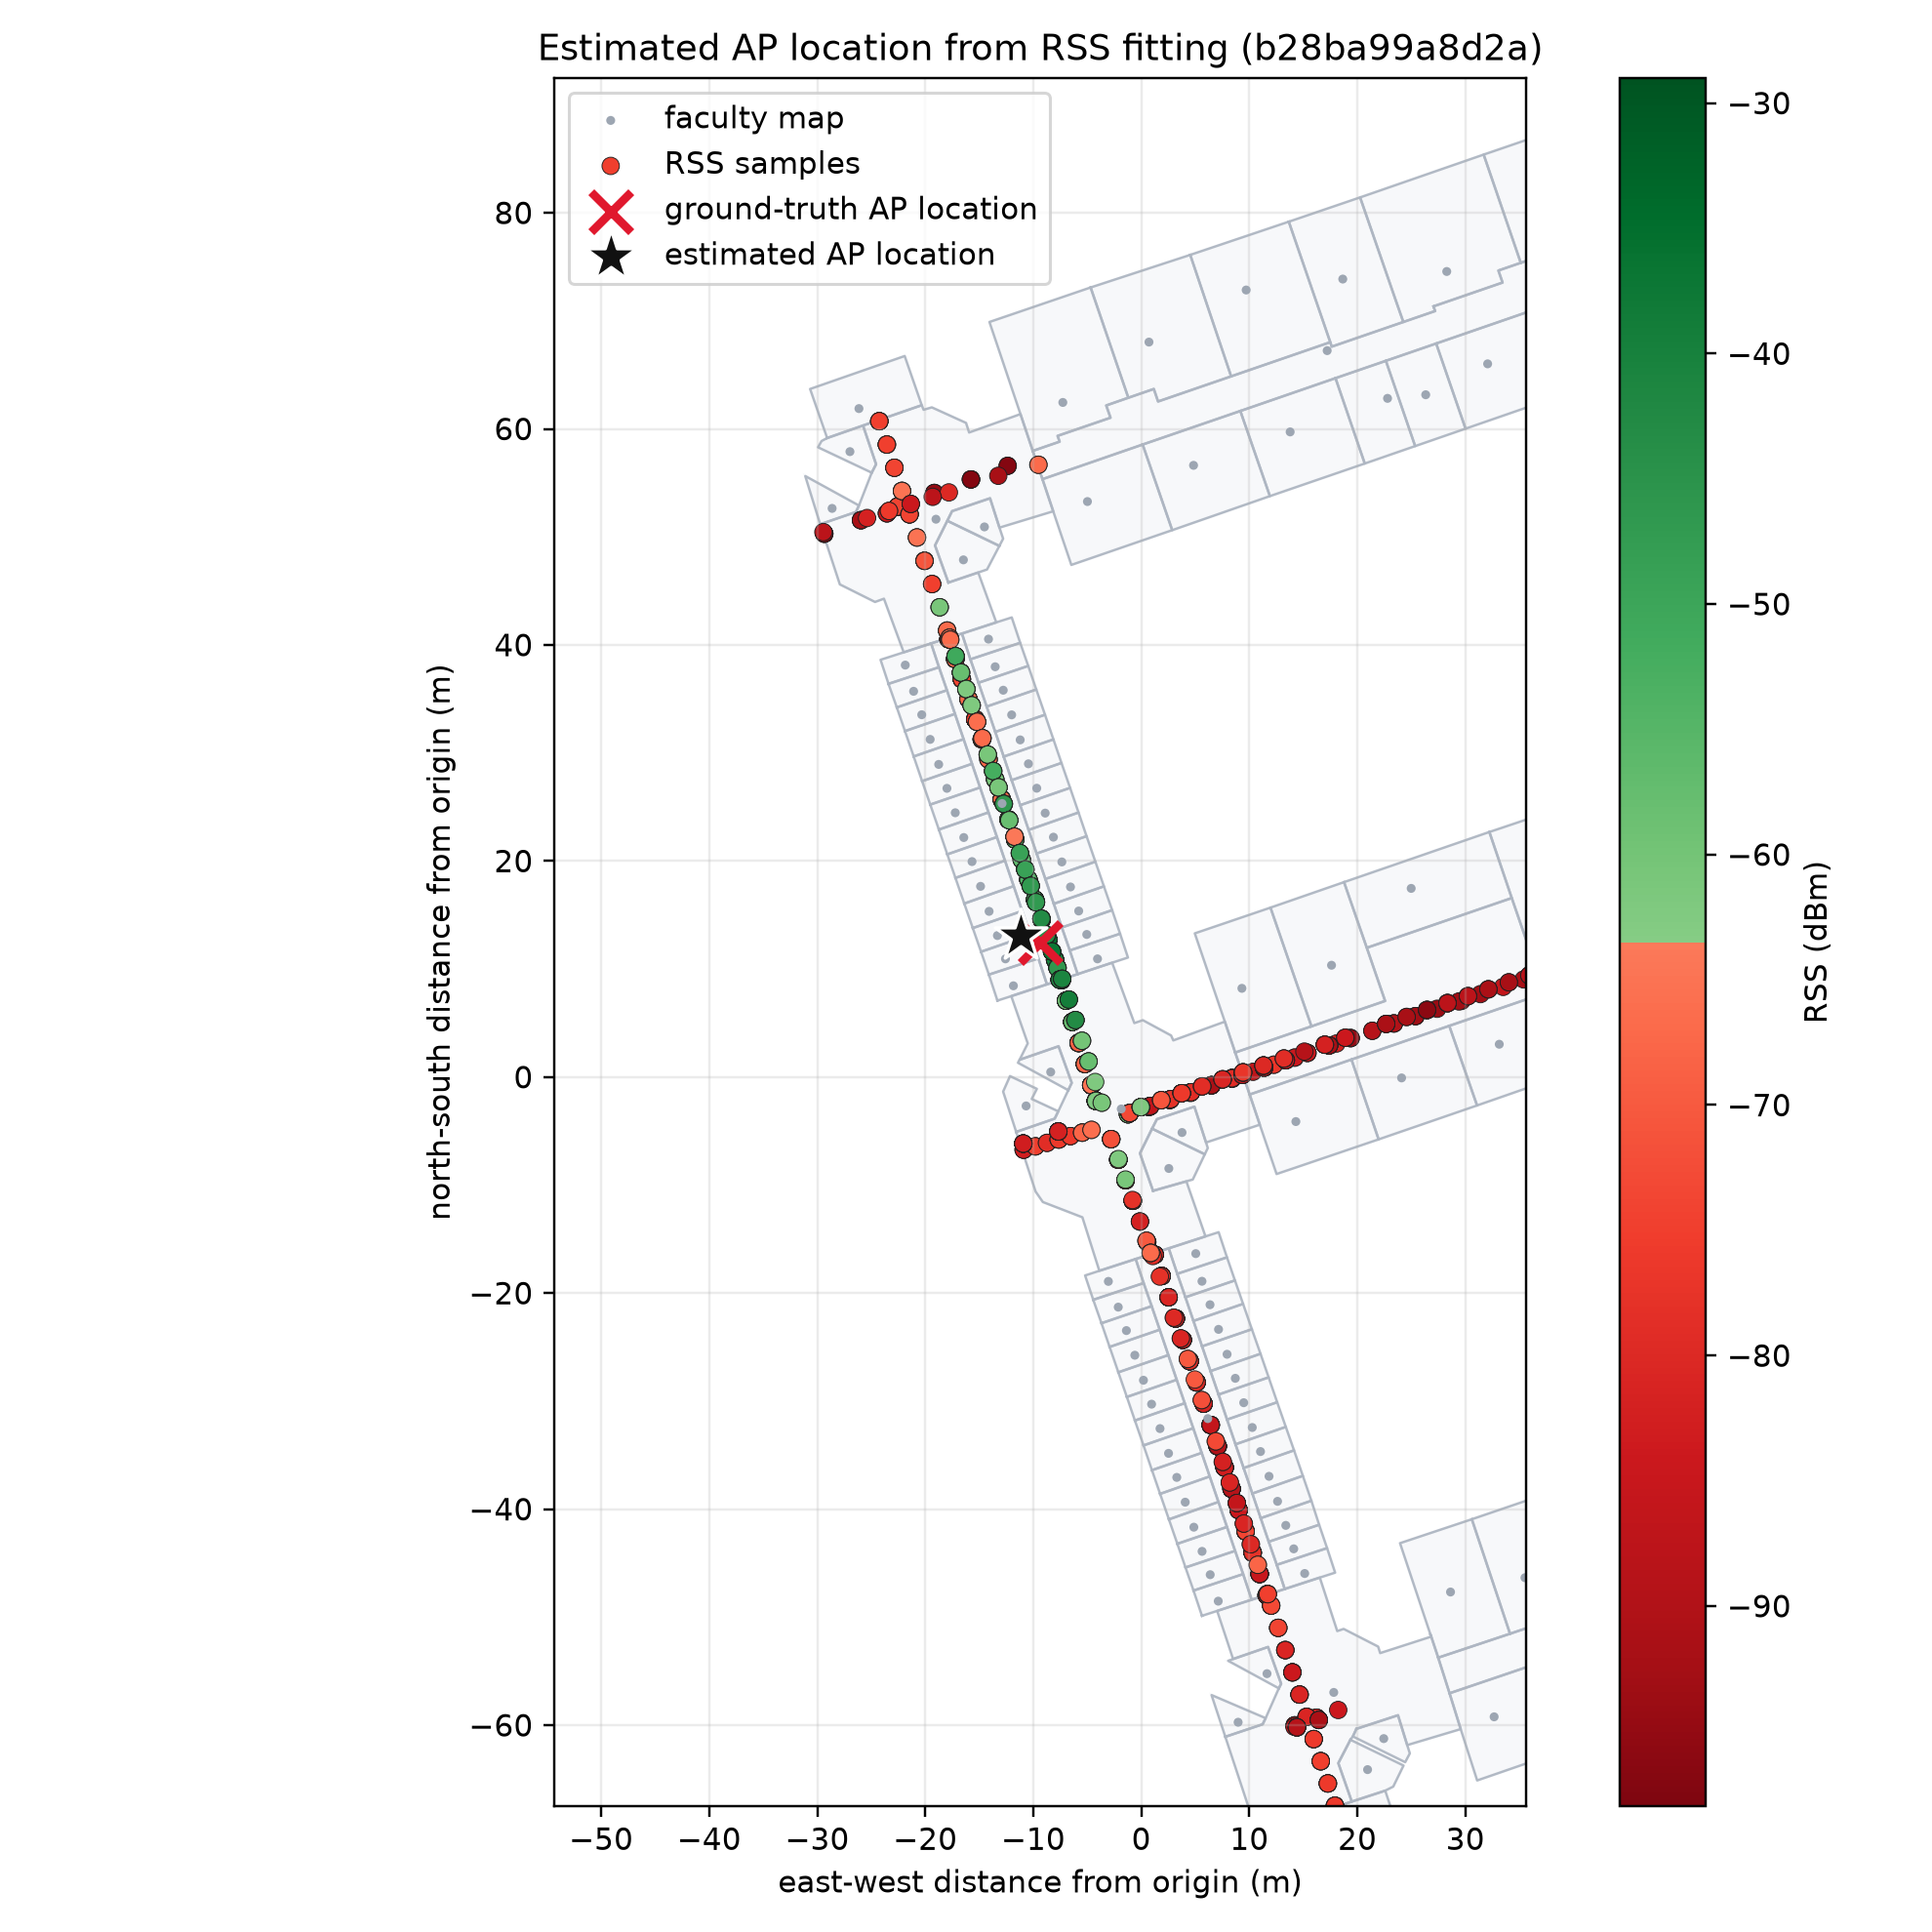
\includegraphics[width=0.82\textwidth]{figures/03_estimated_ap_map.png}
  \caption{مکان تخمین‌زده‌شده‌ی AP روی نقشه، همراه با نمونه‌های RSS و مکان واقعی برای ارزیابی.}
\end{figure}

\section{کد کامل انتخاب AP}
\begin{latin}
\lstinputlisting[style=pythonstyle,caption={\lr{01\_select\_access\_point.py}}]{code/01_select_access_point.py}
\end{latin}

\section{کد کامل رسم نمونه‌های RSS}
\begin{latin}
\lstinputlisting[style=pythonstyle,caption={\lr{02\_plot\_selected\_ap\_from\_pivot.py}}]{code/02_plot_selected_ap_from_pivot.py}
\end{latin}

\section{کد کامل تخمین مکان AP}
\begin{latin}
\lstinputlisting[style=pythonstyle,caption={\lr{03\_fit\_selected\_ap\_location.py}}]{code/03_fit_selected_ap_location.py}
\end{latin}

\section{کد کامل خواندن و رسم نقشه}
\begin{latin}
\lstinputlisting[style=pythonstyle,caption={\lr{faculty\_map\_json.py}}]{code/faculty_map_json.py}
\end{latin}

\section{نکات مهم استخراج‌شده از کد}
\begin{itemize}
  \item فایل‌های train/test در workflow فعلی استفاده نمی‌شوند؛ ورودی اصلی همان جدول pivot است.
  \item مقدار ground-truth فقط برای گزارش خطای نهایی است و وارد optimizer نمی‌شود.
  \item نقطه‌ی شروع optimizer نمونه‌ای است که بیشترین RSS را دارد.
  \item loss از نوع \lr{soft\_l1} است، بنابراین برازش نسبت به نویز و نقاط پرت مقاوم‌تر از least squares معمولی است.
  \item مدل دیوارها، جهت گوشی، چندمسیره‌بودن سیگنال و تفاوت دستگاه‌ها را صریحاً مدل نمی‌کند؛ همه‌ی این اثرها در باقیمانده‌ی مدل جذب می‌شوند.
\end{itemize}

\end{document}
